\documentclass[12pt]{article}
\usepackage[utf8]{inputenc}
\usepackage{amsmath}
\usepackage{graphicx}
\usepackage{float}
\usepackage[margin=1in]{geometry}
\usepackage{lineno}
\setlength{\parindent}{4em}
\setlength{\parskip}{1em}
\renewcommand{\baselinestretch}{1.5}
\newcommand\dbyd[2]{\frac{\mathrm d{#1}}{\mathrm d{#2}}}
\newcommand\dsided[2]{{\mathrm d{#1}}/{\mathrm d{#2}}}
\newcommand{\R}{\mathcal{R}}
\title{Intentional infection as a method of\\population-level disease
  control\\I.~Intentional infection of newborns (Draft)}
\author{Roger Zhang}
\date{June 7th 2018}
\usepackage{color}
\newcommand{\david}[1]{\textcolor{blue}{$\langle${\slshape{\bfseries David:} #1 }$\rangle$}}
\newcommand{\roger}[1]{\textcolor{red}{$\langle${\slshape{\bfseries Roger:} #1 }$\rangle$}}
\usepackage[colorlinks=true,linkcolor=blue]{hyperref}
\newcommand{\pmV}{p_{V}}
\newcommand{\pmI}{p_{I}}


\begin{document}
\maketitle
\begin{abstract}
In this paper, we study the possible advantage of intentional infection. It is a generalized version of variolation, which was invented in 15th century, and widely used around the world in 17th and 18th century. People believed that by variolation, a mild but protective infection would result, which give them a higher chance of survival compared to being normally infected. This paper aims to provide a mathematical model which describes the dynamics of infected classes, when intentional infection is introduced on a population level, and perform predictions based on the model.
\end{abstract}
\tableofcontents

\section{Introduction}
In history, before vaccination became a developed technology, humanity has limited power when facing viral infection. Intentional infection however, act as a precursor of vaccination, was introduced long ago. Although people did not fully understand the detailed mechanism of intentional infections before modern centuries, this method was used extensively to battle some deadly disease, smallpox as a famous representative.\\
There are different strategies in vaccination. Some vaccinations are applied to younglings, for example, polio. Other vaccination may be applied to adults, such as flu vaccination. In fact, same strategies may be translated to intentional infection usage as well.

In this paper, we developed and analyzed a compartmental model, which
coupled direct intentional infection and transmission of intentionally infected cases.
\section{Model: Modification to SIR model}
\subsection{System of differential equations}
We begin our analysis by modifying SIR model. Our first strategy is to intentionally infect newborn individuals, with a certain proportion.  The following assumptions are made to simplify the model to start with:
\begin{itemize}
\item There is no difference between intentionally infected and normally infected individuals.
\item There is no disease induced mortality.
\item Birth and natural death rate are the same, so the total population remains constant.
\item The latent period is short enough to be ignored.
\item All susceptible individuals are equally likely to be infected, and all infected individuals are equally infectious.
\end{itemize}
Equipped with the assumptions above, we now setup our system of differential equations.

Just like in SIR model, $S$, $I$ and $R$ represent the proportion of susceptible, infected and recovered with respect to total population.
\begin{equation}\label{1}
\begin{split}
\dbyd{S}{t}&=\mu(1-p)- \beta SI-\mu S \,,\\
\dbyd{I}{t}&=\beta SI+\mu p-\gamma I -\mu I\,,\\
\dbyd{R}{t}&=\gamma I-\mu R\,.
\end{split}
\end{equation}
Here, $\beta$ is the transmission rate, $\gamma$ is the recovery rate,
$\mu$ is the \emph{per capita} rate of birth and death, $p$ is the
proportion of newborns that are intentionally infected.

We non-dimensionalize \autoref{1} by scaling time, by
\begin{equation}
\tau=(\gamma+\mu)t \,,
\end{equation}
which yields
\begin{subequations}\label{3}
\begin{align}
\dbyd{S}{\tau}&=\epsilon(1-p)- \R_0  SI-\epsilon S \,,\\
\dbyd{I}{\tau}&=\R_0 SI+\epsilon p-I \,,
\end{align}
\end{subequations}
where $\epsilon=\frac{\mu}{\gamma+\mu}$, $\R_0=\frac{\beta}{\gamma+\mu}$.

We are not considering $\dbyd{R}{\tau}$ since it does not impact the dynamics of $S$ or $I$, and we do not need to track the proportion of recovered individuals in this model.
\subsection{Equilibria}
By letting \autoref{3} equal to 0, we solve for equilibria. The only equilibrium for this model is,
\begin{subequations}
\begin{align}
\hat{S} &=\frac{1}{\R_0}-\frac{2p}{(\R_0 -1)+ \sqrt{(\R_0-1)^2+4\R_0 p}}\,, \label{Shat1}\\
\hat{I} &= \frac{\epsilon(\R_0 -1)+ \epsilon \sqrt{(\R_0-1)^2+4\R_0
    p}}{2\R_0}\,.\label{Ihat1}
\end{align}
\end{subequations}

Notice \autoref{Ihat1} does not return 0 for any $p$ value between 0 and 1, it means there is always infected individuals present in the population. Therefore, we can claim that this is not a disease free equilibrium. It follows that the equilibrium above is an endemic equilibrium (EE).

We would like to know if the EE is stable, therefore we need the Jacobian matrix of \autoref{3}. The Jacobian is, 
\begin{equation}
\mathcal{J} =
\begin{bmatrix}
    \ -\R_0 I-\epsilon       & -\R_0 S \\
    \ \R_0 I       & \R_0 S-1 \\
\end{bmatrix} \,.
\end{equation}

Now for simplicity, let 
\begin{equation}\label{E:}
K = (\R_0 -1)+ \sqrt{(\R_0-1)^2+4\R_0 p} \,.
\end{equation}

Notice, $K>0$ if $p\neq 0$.

Thus, the Jacobian evaluated at endemic equilibrium is,
\begin{equation}
\mathcal{J}|_{EE} =
\begin{bmatrix}
    \ -\frac{\epsilon K}{2}-\epsilon       & -1+\frac{2p \R_0}{K} \\
    \ \frac{\epsilon K}{2}       & -\frac{2p \R_0}{K} \\
\end{bmatrix} \label{Jacobian1} \,,
\end{equation}

The eigenvalues of \autoref{Jacobian1} are,
\begin{equation}
\lambda_{1,2} = \frac{-(\epsilon K^2+2\epsilon K +4p\mathcal{R}_0) \pm \sqrt{(\epsilon K^2+2\epsilon K +4p\mathcal{R}_0)^2-4(2\epsilon K^3+8\epsilon Kp\mathcal{R}_0)}}{4K}
\end{equation}

Since $(2\epsilon K^3+8\epsilon Kp\mathcal{R}_0)>0$, therefore, if the discriminant is positive, we have
\begin{equation}
\sqrt{(\epsilon K^2+2\epsilon K +4p\mathcal{R}_0)^2-4(2\epsilon
  K^3+8\epsilon Kp\mathcal{R}_0)}
 \leq|\epsilon K^2+2\epsilon K +4p\mathcal{R}_0|  \,,
\end{equation}

thus, $\Re(\lambda_{1,2})<0$.

But if the discriminant is negative, we have
\begin{equation}
\Re(\lambda_1)=\Re(\lambda_2)=-(\epsilon K^2+2\epsilon K +4p\mathcal{R}_0)<0  \,,
\end{equation}

Therefore, we can conclude that EE is stable.

To fully investigate the dynamics of the system, we're also interested in whether the eigenvalues could be complex, which will lead to damped oscillation. 

Although it is hard to determine the sign of discriminant analytically, we can plot the value of discriminant as a function of other parameter, i.e. $p$ or $\R_0$.

We will start our analysis with specific values of each parameter. Given the variolation history of smallpox, it is reasonable to adopt its parameter values as an example. The values are listed in \autoref{tab:params}.

\begin{table}[H]
\begin{center}
\caption{Model parameters and smallpox values.}
\label{tab:params}
\smallskip
\begin{tabular}{c|c|r}
{\bfseries Symbol} & {\bfseries Meaning} & {\bfseries Value} \\\hline
$\mu$ & Natural \emph{per capita} death rate & $\frac{1}{50*365}$ per day \\
$\gamma$ & Recovery rate & $\frac{1}{22}$ per day \\
$\R_0$ & Basic reproductive number & 4.5
\end{tabular}
\end{center}
\end{table}

\subsection{Dependence of discriminant on proportion intentionally infected ($p$)}
\begin{figure}[H]
  \caption{Discriminant as a function of $p$.}
  \centering
  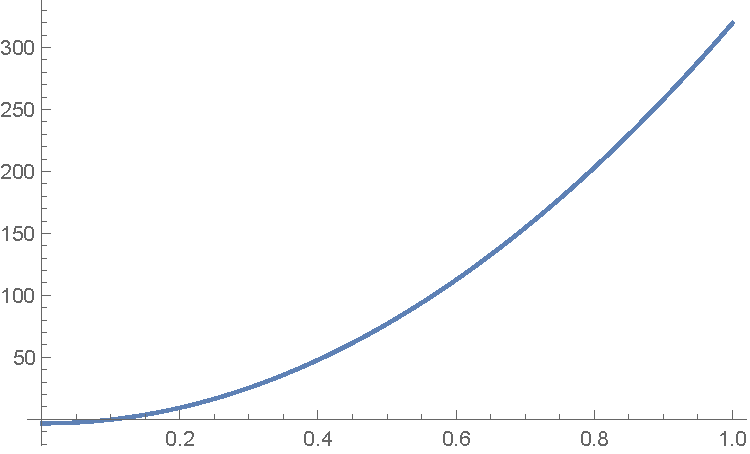
\includegraphics[width=1\textwidth]{Figures/Discriminant_plot_newborn.pdf}
\end{figure}

The $p$-intercept of this graph is $p=0.104$. Meaning, with a proportion of 10.4 percent or less, there is going to be a damped oscillation. In general, a smaller  proportion of intentional infection will lead to damped oscillation.



\subsection{Dependence of discriminant on basic reproduction number ($\R_0$)}

In general, it is often the case where people have limited resources and ability to apply medical treatment, therefore, when an alien pathogen is introduced to a population, it is interesting to see the effect of $\R_0$ on discriminant.

By using values in \autoref{tab:params} except $\R_0$, the following plots are made.

\begin{figure}[H] 
  \caption{Plot discriminant with $\R_0$ to be the variable.$p=0.1$, the $R_0$ -intercept is $\R_0 = 0, 5.75$}
  \centering
  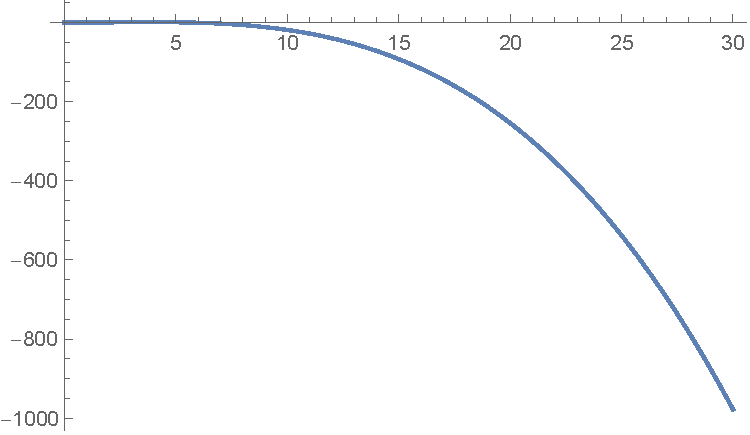
\includegraphics[width=1\textwidth]{Figures/Plot_R_0_p_0_1.pdf}
\end{figure}

\begin{figure}[H] \label{plot:R_0}
  \caption{Plot discriminant with $\R_0$ to be the variable. With $p=0.2$ for the top panel and $p=0.3$ for the bottom panel, the $\R_0$ -intercept is $\R_0 = 0, 17.05$ for the top panel, $\mathcal{R}_0 = 0, 37.45$ for the bottom panel}
  \centering
  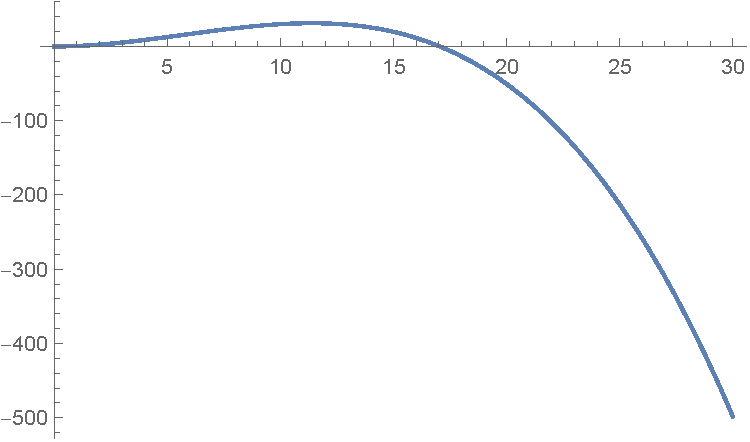
\includegraphics[width=0.9\textwidth]{Figures/Plot_R_0_p_0_2.pdf}
  \centering
  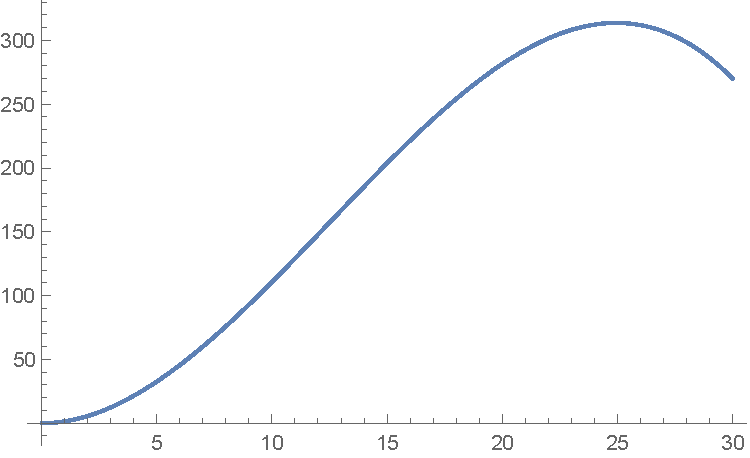
\includegraphics[width=0.85\textwidth]{Figures/Plot_R_0_p_0_3.pdf}
\end{figure}

\autoref{plot:R_0} tells us, With the proportion of intentional infection $p>0.3$, the system has no damped oscillation for a reasonable value of $\R_0$. But for lower $p$, the system tends to have damped oscillation if $\R_0$ is larger.

\subsection{Comments and discussion on this model}
This is the initial model of intentional infection on newborns, compare to vaccination model, the main difference is the whereabouts of the individuals being treated with intentional infection or vaccination. Intentional infected individuals are capable of infecting susceptibles whereas the vaccinated individuals will enter $R$, which is recovered individuals, and not able to impact the dynamics of the system anymore. In ideal cases, once an individual is intentionally infected, either directly or infected by others of the same kind, this individual will not be normally infected anymore. Therefore, we should divide infected compartment into 2 new groups, namely, intentionally infected cases and normally infected cases.

In the past, people believed that ones being intentionally infected would have a lower fatality rate, in comparison with normally infected cases. One way of defining "have advantages" would be comparing total disease induced mortality. Therefore, we need to involve a new parameter, namely, disease induced mortality rate.

\section{Model: Addition of disease induced mortality rate}
\subsection{System of differential equations}
Historic application of variolation have shown that intentional infection has a lower mortality rate in comparison with being normally infected. Therefore, we need to assign different mortality rate to each classes. That also require us to divide $I$ from our previous model into two distinct infected classes. Here, we call them "Intentionally infected" ($V$) and "Normally infected" ($I$). 

With all other assumptions still being valid, we have to remove the first one, which claimed intentionally and normally infected cases have no difference.

Therefore, our model becomes,
\begin{equation}\label{2}
\begin{split}
\dbyd{S}{t}&=\mu(1-p)- \beta S(V+I)-\mu S \,,\\
\dbyd{V}{t}&=\beta SV+\mu p-\gamma V -\mu V\,,\\
\dbyd{I}{t}&=\beta SI-\gamma I -\mu I\,,\\
\dbyd{M}{t}&=\pmV\gamma V+\pmI\gamma I\,,\\
\dbyd{R}{t}&=(1-\pmV)\gamma V+(1-\pmI)\gamma I-\mu R\,,
\end{split}
\end{equation}

In addition to the previous model, $\pmV$ and $\pmI$ represent the mortality rate for intentionally infected and normally infected cases, respectively.

Again, we non-dimensionalize \autoref{2} by time, by
\begin{equation}
\tau=(\gamma+\mu)t \,,
\end{equation}
which yields,
\begin{subequations}\label{eq:base_ODE}
\begin{align}
\dbyd{S}{\tau}&=\epsilon(1-p)- \R_0 S(V+I)-\epsilon S\,, \label{eq:S_by_tau}\\
\dbyd{V}{\tau}&=\R_0 SV+\epsilon p-V\,, \label{eq:V_by_tau}\\
\dbyd{I}{\tau}&=\R_0 SI-I\,, \label{eq:I_by_tau}\\
\dbyd{M}{\tau}&=\pmV(1-\epsilon) V+\pmI(1-\epsilon) I\,,\\
\dbyd{R}{\tau}&=(1-\pmV)(1-\epsilon) V+(1-\pmI)(1-\epsilon) I-\epsilon R\,,
\end{align}
\end{subequations}

\subsection{Equilibria}

By letting \autoref{eq:S_by_tau}, \autoref{eq:V_by_tau} and \autoref{eq:I_by_tau} equal to 0, we solve for solutions.

If $p=0$, meaning there is no intentional infection, then the equilibrium is the standard equilibrium for SIR model, which is,
\begin{subequations}
\begin{align}
\hat{S} &= \frac{1}{\R_0}\,,\\
\hat{V} &= 0\,,\\
\hat{I} &= \epsilon(1-\frac{1}{\R_0})\,.
\end{align}
\end{subequations}

Or,
\begin{subequations}
\begin{align}
\hat{S} &= 1\,,\\
\hat{V} &= 0\,,\\
\hat{I} &= 0\,.
\end{align}
\end{subequations}

However, if $p\neq 0$, the equilibrium is,
\begin{subequations}
\begin{align}
\hat{S}&= \frac{1}{\R_0}-\frac{2p}{(\R_0 -1)+ \sqrt{(\R_0-1)^2+4\R_0
         p}}\,, \label{eq:Shat}\\
\hat{V}&= \frac{\epsilon(\R_0 -1)+ \epsilon \sqrt{(\R_0-1)^2+4\R_0 p}}{2\R_0}\,, \label{eq:Vhat}\\
\hat{I}&=0\,. \label{eq:Ihat}
\end{align}
\end{subequations}

Since $\hat{V}\neq 0$, for any $p$ between 0 and 1, this equilibrium is not disease free. It follows that this equilibrium is the endemic equilibrium.

Stability analysis relies on Jacobian matrix, which is,
\begin{equation}
\mathcal{J} =
\begin{bmatrix}
    \ -\R_0 (V+I)-\epsilon       & -\R_0 S     &-\R_0 S\\
    \ \R_0 V       & \R_0 S-1    &0\\
    \ \R_0 I       &0     &\R_0 S-1\\
\end{bmatrix}\,.
\end{equation}

Eigenvalues of Jacobian are given as follow,
\begin{subequations}
\begin{align}
\lambda_1&=-1+\R_0 S \label{eq:lambda1}\\
\lambda_2&=\frac{-1+\R_0 S-\epsilon-\R_0 V-\sqrt{(-1+\R_0 S-\epsilon-\R_0 V)^2-4(\R_0+\epsilon-\R_0 S\epsilon)}}{2} \label{eq:lambda2}\\
\lambda_3&=\frac{-1+\R_0 S-\epsilon-\R_0 V+\sqrt{(-1+\R_0 S-\epsilon-\R_0 V)^2-4(\R_0+\epsilon-\R_0 S\epsilon)}}{2}\label{eq:lambda3}
\end{align}
\end{subequations}

By using \autoref{eq:Shat} and \autoref{eq:lambda1}, we obtain
\begin{equation}
-1+\R_0 S = - \frac{2p\R_0}{(\R_0 -1)+ \sqrt{(\R_0-1)^2+4\R_0 p}}<0
\end{equation}
Therefore,
\begin{equation}
\Re(\lambda_1) =-1+\R_0 S<0\,,
\end{equation}
To determine the real part of $\lambda_2$ and $\lambda_3$, we need to determine the sign of the quantity under the square root. 

By using \autoref{eq:Shat} again, we have
\begin{equation}
\R_0 S\epsilon<\epsilon\,,
\end{equation}

Therefore,
\begin{equation}
(\R_0+\epsilon-\R_0 S\epsilon)>\R_0 >0\,,
\end{equation}
which means, if the sign of the quantity under the square root is positive, we necessarily have
\begin{equation}
\sqrt{(-1+\R_0 S-\epsilon-\R_0 V)^2-4(\R_0+\epsilon-\R_0 S\epsilon)}<|(-1+\R_0 S-\epsilon-\R_0 V)|
\end{equation}
Therefore, $\Re(\lambda_2)<\Re(\lambda_3)<0$.

Certainly, if the sign of the quantity under the square root is negative,
\begin{equation}
\Re(\lambda_2)=\Re(\lambda_3)=-1+\R_0 S-\epsilon-\R_0 V<0
\end{equation}

We are able to conclude that EE is stable.

\subsection{Effect of intentional infection in terms of total mortality}

In epidemic analysis, one way of measuring whether a certain method has advantage over another is to compare the total disease induced mortality. 

We first want to mention that, if we look at the mortality rate at EE,
\begin{equation}
\dbyd{M}{\tau}=\pmV(1-\epsilon)V=\frac{\pmV(1-\epsilon)\epsilon(\R_0 -1)+ \pmV(1-\epsilon)\epsilon \sqrt{(\R_0-1)^2+4\R_0 p}}{2\R_0}\,, \label{eq:dMdt}
\end{equation}

An important observation is, at EE, mortality rate increases as $p$ increases. This tells us, in the long run, having a larger proportion of intentional infection is not wise, since it leads extra casualties.

In history, smallpox has a much longer history than variolation, therefore variolation is not immediately invented as smallpox was introduced into human society, but rather appeared at an equilibrium state. So, we are interested in the scenario where intentional infection is only introduced after the population is in equilibrium, with no intentional infection.

We are interested in the time it takes to reach the new EE. Since the new equilibrium has $\hat{I}=0$, we define reaching equilibrium $I\leq 1\times 10^{-6}$ (one in a million).

To help us observe the dynamics better, here we assume variolation mortality rate equal 20 percent.

by plotting, we obtain \autoref{figure:0.0001}
\begin{figure}[h]
  \centering
  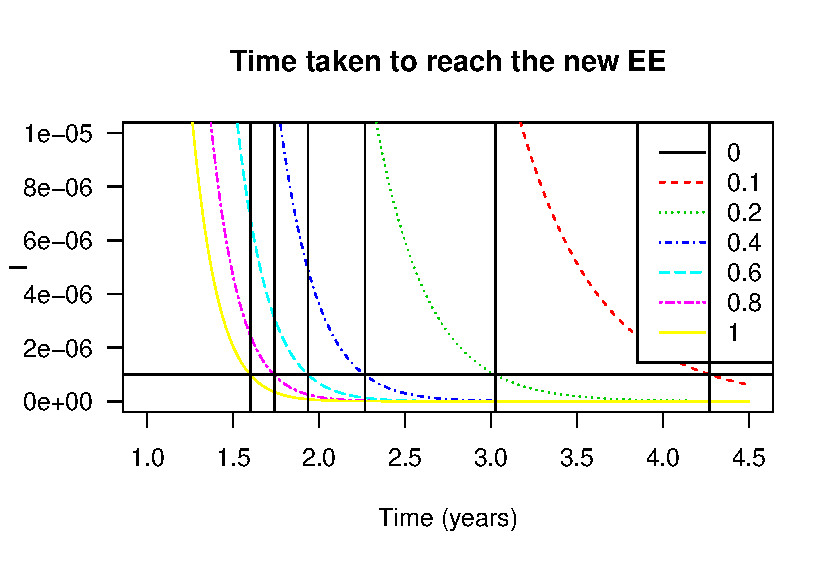
\includegraphics[width=0.9\textwidth]{Figures/I_less_than_0_000001.pdf}
  \caption{Determination of time taken to reach equilibrium}
\label{figure:0.0001}
\end{figure}

We are also interested in the time it takes for intentional infection to take advantage over non-intentional infection, by comparing total mortality.

From previous analysis, we learned that $\dbyd{M}{\tau}$ decreases over time, and stabilizes at a constant rate when reaching the new EE. But at the new EE, $\dbyd{M}{\tau}$ is higher when $p$ is higher. 

\begin{figure}[H]
  \centering
  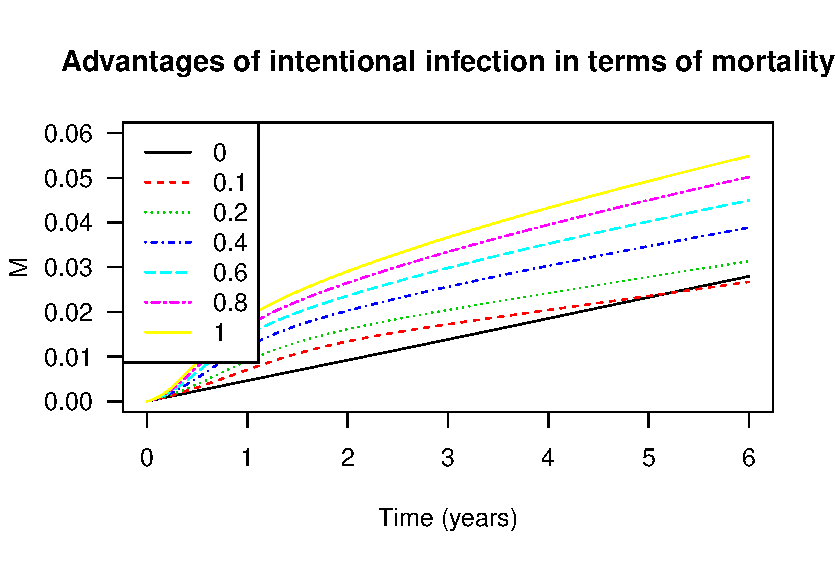
\includegraphics[width=0.9\textwidth]{Figures/dMdt.pdf}
  \caption{An illustration of intentional infection have advantages over non-intentional infection}
\label{figure:advantage}
\end{figure}

\autoref{figure:advantage} shows, at earlier times, intentional infections have steeper slopes than the black line, which is non-intentional infection. The slopes for intentional infection decreases over time, and eventually all of them have smaller slope than the black line.

\autoref{tab:times} summarize the times required to reach the new EE and time required to have advantages over non-intentional infection.

\begin{table}[H]
\begin{center}
\caption{Time required to reach equilibrium and have advantages over non-intentional infection}
\label{tab:times}
\smallskip
\begin{tabular}{c|c|r}
{\bfseries $p$} & {\bfseries Time to EE} & {\bfseries Time to have advantages} \\\hline
0.1 & 4.27 yrs & 5.20 yrs \\
0.2 & 3.03 yrs & 8.81 yrs \\
0.4 & 2.27 yrs & 17.45 yrs \\
0.6 & 1.94 yrs & 28.37 yrs \\
0.8 & 1.74 yrs & 42.43 yrs \\
1.0 & 1.60 yrs & 61.46 yrs
\end{tabular}
\end{center}
\end{table}
The table showed that as $p$ increases, the system reaches the new EE faster, but the time required to have advantages over non-intentional infection increase.

In fact, if $\pmV=0.01$, then the time required to have advantages over non-intentional infection is minimal, and the difference between different $p$ is also insignificant on a scale of years.

\autoref{figure:advantage_by_p} shows us a relationship between time to advantage and $p$.
\begin{figure}[H]
  \centering
  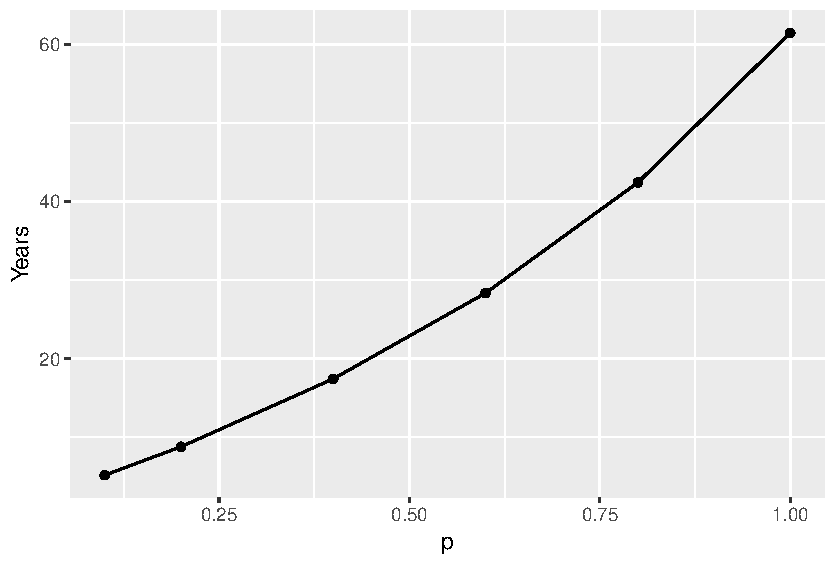
\includegraphics[width=0.9\textwidth]{Figures/time_to_advantage_plot.pdf}
  \caption{Time to advantage, as a function of $p$}
\label{figure:advantage_by_p}
\end{figure}

\subsection{Comments and discussion on this model}

In this model, we have shown that intentional infection has advantages over non-intentional infection in terms of total mortality. However, interestingly, since a larger $p$ will lead to more death in the long run, it is unwise to keep intentional infecting a larger proportion of newborns. 

From \autoref{tab:times} and \autoref{figure:advantage_by_p}, time required to have advantage over non-intentional infection has inverse relationship with $p$. It seems to suggest that we can intentional infect a minimal proportion of newborn, and we are able to optimize total mortality. However, in such case, it will take a much longer time to reach EE, and we can deduce that the initial behavior of mortality will be very close to the black line, though it crosses it and goes beneath in a very short time, but since the slope changes extremely slowly, the difference between intentional infection and non-intentional infection increases at a very slow rate. 

To summarize the above argument, if our strategy of intentional infection remain the same at all time, then in the long run, with a minimal proportion of intentional infection, total mortality could be minimized. However, in real life scenario, strategy does not need to be constant, it may be possible to intentionally infect at a relatively higher proportion initially, and decrease the proportion, or even stop intentional infection, with a combination of strategies like that, we could possibly minimize the total mortality. Or even eradicate the disease.

Other than strategic evolvement, there could still be some development to the model itself to make it more suitable to a realistic scenario. Since Intentional infection has a lower death rate, we could assume a milder symptom for intentionally infected cases. As a result, since aggressive symptoms are typical routes of disease transmission, lack of such pathways will lead to a decrease of transmission rate. Besides, intentionally and normally infected cases could have different recovery rate. Therefore, our next model could consider various possibilities of these parameters, and draw conclusions to its behavior.

\subsection{Possibility of eradication}
If we define the disease been eradicated if the proportion of infected is less than one in a million. Then, our model is able to predict possible eradication of the disease.

At EE, $I=0$, although $I$ is going to approach 0 asymptotically, it will never completely cease to exist. However, we know that there is a point in forward time where $I<1\times10^{-6}$. Therefore, we can claim that normally infected cases could be eradicated.

The next question would be whether it is possible for intentionally infected cases to burn out. After $I$ being wiped out, we could stop intentional infecting any other newborns. From then on if $S<\frac{1}{\R_0}$ for a long enough period of time, which means the effective $\R_0$ is less than 1, we could possibly observe $V<1\times10^{-6}$, which in return, represent the eradication of intentionally infected cases as well.

We use one example to illustrate the occurrence of such scenario. Assume we have $p=1$ until we reach EE. We could calculate $\hat{S}$ and $\hat{I}$. Now if we set the initial condition being the $\hat{S}$ and $\hat{I}$ we just calculated, and let $p=0$, we run the simulation and obtain the following,
\begin{figure}[H]
  \centering
  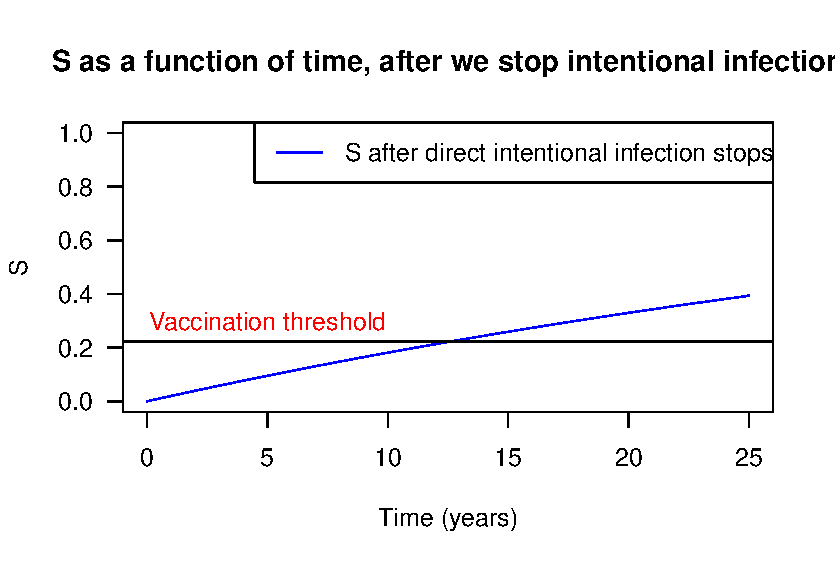
\includegraphics[width=1.1\textwidth]{Figures/Increase_of_S.pdf}
  \caption{For more than 10 years after we stop intentional infection, $S<\frac{1}{\R_0}$}
\label{figure:S_after_stop}
\end{figure}

\begin{figure}[H]
  \centering
  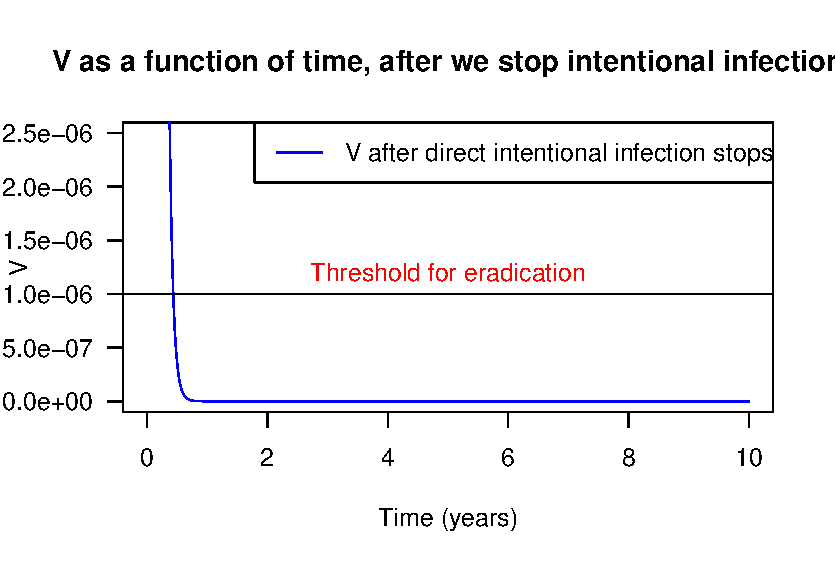
\includegraphics[width=1.1\textwidth]{Figures/V_after_stop.pdf}
  \caption{It takes less than 1 year for $V$ to fall below $1\times10^{-6}$}
\label{figure:V_after_stop}
\end{figure}

\autoref{figure:S_after_stop} and \autoref{figure:V_after_stop} have shown an example of disease eradication, by our definition. Other values of $p$ will still need to be investigated.

\section{Model: Different transmission rate and recovery rate}
\subsection{System of differential equations}
As we mentioned above, we need to involve new parameters for different transmission and recovery rate. Here, we let $\beta_V$ and $\beta_I$ represent the transmission rate of variolated cases and pathogen infected cases, respectively. $\gamma_V$ and $\gamma_I$ are the recovery rate of variolated cases and pathogen infected cases, respectively.

With the new parameters in hand, we now setup our system of differential equation,
\begin{equation}\label{model:complex}
\begin{split}
\dbyd{S}{t}&=\mu(1-p)- \beta_V SV -\beta_I SI-\mu S \,,\\
\dbyd{V}{t}&=\beta_V SV+\mu p-\gamma_V V -\mu V\,,\\
\dbyd{I}{t}&=\beta_I SI-\gamma_I I -\mu I\,,\\
\dbyd{M}{t}&=\pmV\gamma_V V+\pmI\gamma_I I\,,\\
\dbyd{R}{t}&=(1-\pmV)\gamma_V V+(1-\pmI)\gamma_I I-\mu R\,,
\end{split}
\end{equation}

We non-dimensionalize \autoref{model:complex} by scaling time, by
\begin{equation}
\tau=(\gamma_I+\mu)t \,,
\end{equation}

As the result, we obtain,
\begin{subequations}\label{eq:base_ODE}
\begin{align}
\dbyd{S}{\tau}&=\epsilon(1-p)-\R_{0,V} SV-\R_{0,I} SI-\epsilon S\,, \label{eq:S_by_tau}\\
\dbyd{V}{\tau}&=\R_{0,V} SV+\epsilon p-\tilde{\gamma} V\,, \label{eq:V_by_tau}\\
\dbyd{I}{\tau}&=\R_{0,I} SI-I\,, \label{eq:I_by_tau}\\
\dbyd{M}{\tau}&=\pmV(\tilde{\gamma}-\epsilon) V+\pmI(1-\epsilon) I\,,\\
\dbyd{R}{\tau}&=(1-\pmV)(\tilde{\gamma}-\epsilon) V+(1-\pmI)(1-\epsilon) I-\epsilon R\,,
\end{align}
\end{subequations}

Where $\R_{0,V}=\frac{\beta_V}{\gamma_I+\mu}$, $\R_{0,I}=\frac{\beta_I}{\gamma_I+\mu}$, $\tilde{\gamma}=\frac{\gamma_V+\mu}{\gamma_I+\mu}$, $\epsilon=\frac{\mu}{\gamma_I+\mu}$.

\subsection{Equilibria}

To solve for all equilibria, we let equations \autoref{eq:S_by_tau}, \autoref{eq:V_by_tau} and \autoref{eq:I_by_tau} equal to 0, we solve for solutions.

We acquired three sets of solutions. However, given conditions that all $\hat{S}$, $\hat{V}$ and $\hat{I}$ have to be a non-negative number between 0 and 1, we can discard two of the solutions, and the only set of solution left is, 
\begin{subequations}
\begin{align}
\hat{S}&= \frac{\R_{0,V}+\tilde{\gamma}-\sqrt{\R_{0,V}^2-2\R_{0,V}\tilde{\gamma}+\tilde{\gamma}^2+4p\R_{0,V}\tilde{\gamma}}}{2\R_{0,V}}\,, \label{eq:Shat}\\
\hat{V}&= \frac{\epsilon-\frac{\tilde{\gamma}\epsilon}{\R_{0,V}}+\frac{\epsilon\sqrt{\R_{0,V}^2-2\R_{0,V}\tilde{\gamma}+\tilde{\gamma}^2+4p\R_{0,V}\tilde{\gamma}}}{\R_{0,V}}}{2\tilde{\gamma}}\,, \label{eq:Vhat}\\
\hat{I}&=0\,, \label{eq:Ihat}
\end{align}
\end{subequations}

Similar to our previous models, since infected population at equilibrium is non-zero, this is not a disease free equilibrium but rather an endemic equilibrium.

Stability analysis rely on Jacobian Matrix,
\begin{equation}
\mathcal{J} =
\begin{bmatrix}
    \ -\R_{0,V}V-\R_{0,I}I-\epsilon       & -\R_{0,V}S     &-\R_{0,I}S\\
    \ \R_{0,V}V       & \R_{0,V}S-\gamma    &0\\
    \ \R_{0,I}I       &0     &\R_{0,I} S-1\\
\end{bmatrix}\,.
\end{equation}

Eigenvalues of Jacobian are given as follow,
\begin{subequations}
\begin{align}
\lambda_1&=-1+\R_{0,I} S \label{eq:lambda1}\\
\lambda_2&=\frac{-\tilde{\gamma}+\R_{0,V}S-\epsilon-\R_{0,V}V-\sqrt{(-\tilde{\gamma}+\R_{0,V} S-\epsilon-\R_{0,V}V)^2-4(\R_{0,V}\tilde{\gamma}+\epsilon\tilde{\gamma}-\R_{0,V}S\epsilon)}}{2} \label{eq:lambda2}\\
\lambda_3&=\frac{-\tilde{\gamma}+\R_{0,V}S-\epsilon-\R_{0,V}V+\sqrt{(-\tilde{\gamma}+\R_{0,V} S-\epsilon-\R_{0,V}V)^2-4(\R_{0,V}\tilde{\gamma}+\epsilon\tilde{\gamma}-\R_{0,V}S\epsilon)}}{2}\label{eq:lambda3}
\end{align}
\end{subequations}

By using \autoref{eq:Shat}, we know that
\begin{equation}
0\leq S\leq \frac{\tilde{\gamma}}{\R_{0,V}}\,.{\label{middle}}
\end{equation}
Therefore, 
\begin{equation}
\Re(\lambda_1) <0
\end{equation}
iff 
\begin{equation}
\frac{\tilde{\gamma}}{\R_{0,V}}<\frac{1}{\R_{0,I}}
\end{equation}

Or equivalently 
\begin{equation}
\frac{\beta_V}{\beta_I}<\tilde{\gamma}^2
\end{equation}
Intuitively, if recovery rate are similar for variolated and normally infected cases, i.e. $\tilde{\gamma}\approx 1$, the endemic equilibrium is unstable if $\R_{0,V}<\R_{0,I}$

For the real part of $\lambda_2$ and $\lambda_3$, first we look at the terms before square root. 

By using \autoref{middle}, we have
\begin{equation}
-\tilde{\gamma}+\R_{0,V}S-\epsilon-\R_{0,V}V<0\,,
\end{equation}

Therefore,
\begin{equation}
\Re(\lambda_2)<-\tilde{\gamma}+\R_{0,V}S-\epsilon-\R_{0,V}V<0\,,
\end{equation}

Next, notice
\begin{equation}
\R_{0,V}\tilde{\gamma}+\epsilon\tilde{\gamma}-\R_{0,V}S\epsilon>0\,.
\end{equation}
It follows that
\begin{equation}
\sqrt{(-\tilde{\gamma}+\R_{0,V} S-\epsilon-\R_{0,V}V)^2-4(\R_{0,V}\tilde{\gamma}+\epsilon\tilde{\gamma}-\R_{0,V}S\epsilon)}<|-\tilde{\gamma}+\R_{0,V} S-\epsilon-\R_{0,V}V|
\end{equation}
Therefore, $\Re(\lambda_3)<0$.

As a result, we cannot directly conclude the stability of EE, but we have observed that stability depends on $\tilde{\gamma}$ and $\R_{0,I}$

\subsection{Comments and discussion on this model}

Parameters of this model such as $\R_{0,V}$ and $\gamma_V$ are custom to the design of pathogen used for intentional infection. 

Previous study have shown that, for a similar model which does not consider death, a significant decrease in final size is expected, for a transmissible vaccine, even when $\R_{0,V}$ is less than 1, e.g. $\R_{0,V}=0.5$, we would expect similar results for our model, the difference is, with the addition of birth and death rate, since our system have shown that the disease cannot be completely eradicated, there will always be newly infected cases, therefore, we do not have a final size estimation. 

If one tries to make a fast vaccine (high transmission rate and fast recovery rate), we would expect a bigger $\beta_V$ and $\tilde{\gamma}$ value, $\R_{0,V}$ is indeterminate.

\section{Future work}
This section elaborates some ideas for future use and needs to be investigated later.
\begin{itemize}
\item Comparison between intentional infection and traditional vaccine, which does not transmit. This is for showing intentional infection as a more effective method to vaccinate.
\end{itemize}

\end{document}
